\documentclass[]{article}
\usepackage{lmodern}
\usepackage{amssymb,amsmath}
\usepackage{ifxetex,ifluatex}
\usepackage{fixltx2e} % provides \textsubscript
\ifnum 0\ifxetex 1\fi\ifluatex 1\fi=0 % if pdftex
  \usepackage[T1]{fontenc}
  \usepackage[utf8]{inputenc}
\else % if luatex or xelatex
  \ifxetex
    \usepackage{mathspec}
  \else
    \usepackage{fontspec}
  \fi
  \defaultfontfeatures{Ligatures=TeX,Scale=MatchLowercase}
\fi
% use upquote if available, for straight quotes in verbatim environments
\IfFileExists{upquote.sty}{\usepackage{upquote}}{}
% use microtype if available
\IfFileExists{microtype.sty}{%
\usepackage{microtype}
\UseMicrotypeSet[protrusion]{basicmath} % disable protrusion for tt fonts
}{}
\usepackage[margin=1in]{geometry}
\usepackage{hyperref}
\hypersetup{unicode=true,
            pdftitle={BST169: Course Work Project answer},
            pdfauthor={sn0wfree},
            pdfborder={0 0 0},
            breaklinks=true}
\urlstyle{same}  % don't use monospace font for urls
\usepackage{color}
\usepackage{fancyvrb}
\newcommand{\VerbBar}{|}
\newcommand{\VERB}{\Verb[commandchars=\\\{\}]}
\DefineVerbatimEnvironment{Highlighting}{Verbatim}{commandchars=\\\{\}}
% Add ',fontsize=\small' for more characters per line
\usepackage{framed}
\definecolor{shadecolor}{RGB}{248,248,248}
\newenvironment{Shaded}{\begin{snugshade}}{\end{snugshade}}
\newcommand{\KeywordTok}[1]{\textcolor[rgb]{0.13,0.29,0.53}{\textbf{{#1}}}}
\newcommand{\DataTypeTok}[1]{\textcolor[rgb]{0.13,0.29,0.53}{{#1}}}
\newcommand{\DecValTok}[1]{\textcolor[rgb]{0.00,0.00,0.81}{{#1}}}
\newcommand{\BaseNTok}[1]{\textcolor[rgb]{0.00,0.00,0.81}{{#1}}}
\newcommand{\FloatTok}[1]{\textcolor[rgb]{0.00,0.00,0.81}{{#1}}}
\newcommand{\ConstantTok}[1]{\textcolor[rgb]{0.00,0.00,0.00}{{#1}}}
\newcommand{\CharTok}[1]{\textcolor[rgb]{0.31,0.60,0.02}{{#1}}}
\newcommand{\SpecialCharTok}[1]{\textcolor[rgb]{0.00,0.00,0.00}{{#1}}}
\newcommand{\StringTok}[1]{\textcolor[rgb]{0.31,0.60,0.02}{{#1}}}
\newcommand{\VerbatimStringTok}[1]{\textcolor[rgb]{0.31,0.60,0.02}{{#1}}}
\newcommand{\SpecialStringTok}[1]{\textcolor[rgb]{0.31,0.60,0.02}{{#1}}}
\newcommand{\ImportTok}[1]{{#1}}
\newcommand{\CommentTok}[1]{\textcolor[rgb]{0.56,0.35,0.01}{\textit{{#1}}}}
\newcommand{\DocumentationTok}[1]{\textcolor[rgb]{0.56,0.35,0.01}{\textbf{\textit{{#1}}}}}
\newcommand{\AnnotationTok}[1]{\textcolor[rgb]{0.56,0.35,0.01}{\textbf{\textit{{#1}}}}}
\newcommand{\CommentVarTok}[1]{\textcolor[rgb]{0.56,0.35,0.01}{\textbf{\textit{{#1}}}}}
\newcommand{\OtherTok}[1]{\textcolor[rgb]{0.56,0.35,0.01}{{#1}}}
\newcommand{\FunctionTok}[1]{\textcolor[rgb]{0.00,0.00,0.00}{{#1}}}
\newcommand{\VariableTok}[1]{\textcolor[rgb]{0.00,0.00,0.00}{{#1}}}
\newcommand{\ControlFlowTok}[1]{\textcolor[rgb]{0.13,0.29,0.53}{\textbf{{#1}}}}
\newcommand{\OperatorTok}[1]{\textcolor[rgb]{0.81,0.36,0.00}{\textbf{{#1}}}}
\newcommand{\BuiltInTok}[1]{{#1}}
\newcommand{\ExtensionTok}[1]{{#1}}
\newcommand{\PreprocessorTok}[1]{\textcolor[rgb]{0.56,0.35,0.01}{\textit{{#1}}}}
\newcommand{\AttributeTok}[1]{\textcolor[rgb]{0.77,0.63,0.00}{{#1}}}
\newcommand{\RegionMarkerTok}[1]{{#1}}
\newcommand{\InformationTok}[1]{\textcolor[rgb]{0.56,0.35,0.01}{\textbf{\textit{{#1}}}}}
\newcommand{\WarningTok}[1]{\textcolor[rgb]{0.56,0.35,0.01}{\textbf{\textit{{#1}}}}}
\newcommand{\AlertTok}[1]{\textcolor[rgb]{0.94,0.16,0.16}{{#1}}}
\newcommand{\ErrorTok}[1]{\textcolor[rgb]{0.64,0.00,0.00}{\textbf{{#1}}}}
\newcommand{\NormalTok}[1]{{#1}}
\usepackage{graphicx,grffile}
\makeatletter
\def\maxwidth{\ifdim\Gin@nat@width>\linewidth\linewidth\else\Gin@nat@width\fi}
\def\maxheight{\ifdim\Gin@nat@height>\textheight\textheight\else\Gin@nat@height\fi}
\makeatother
% Scale images if necessary, so that they will not overflow the page
% margins by default, and it is still possible to overwrite the defaults
% using explicit options in \includegraphics[width, height, ...]{}
\setkeys{Gin}{width=\maxwidth,height=\maxheight,keepaspectratio}
\IfFileExists{parskip.sty}{%
\usepackage{parskip}
}{% else
\setlength{\parindent}{0pt}
\setlength{\parskip}{6pt plus 2pt minus 1pt}
}
\setlength{\emergencystretch}{3em}  % prevent overfull lines
\providecommand{\tightlist}{%
  \setlength{\itemsep}{0pt}\setlength{\parskip}{0pt}}
\setcounter{secnumdepth}{5}
% Redefines (sub)paragraphs to behave more like sections
\ifx\paragraph\undefined\else
\let\oldparagraph\paragraph
\renewcommand{\paragraph}[1]{\oldparagraph{#1}\mbox{}}
\fi
\ifx\subparagraph\undefined\else
\let\oldsubparagraph\subparagraph
\renewcommand{\subparagraph}[1]{\oldsubparagraph{#1}\mbox{}}
\fi

%%% Use protect on footnotes to avoid problems with footnotes in titles
\let\rmarkdownfootnote\footnote%
\def\footnote{\protect\rmarkdownfootnote}

%%% Change title format to be more compact
\usepackage{titling}

% Create subtitle command for use in maketitle
\newcommand{\subtitle}[1]{
  \posttitle{
    \begin{center}\large#1\end{center}
    }
}

\setlength{\droptitle}{-2em}
  \title{BST169: Course Work Project answer}
  \pretitle{\vspace{\droptitle}\centering\huge}
  \posttitle{\par}
  \author{sn0wfree}
  \preauthor{\centering\large\emph}
  \postauthor{\par}
  \predate{\centering\large\emph}
  \postdate{\par}
  \date{11/10/2016}


\begin{document}
\maketitle

{
\setcounter{tocdepth}{2}
\tableofcontents
}
\section{BST169: Course Work Project}\label{bst169-course-work-project}

\subsection{Question 1:}\label{question-1}

\begin{enumerate}
\def\labelenumi{\arabic{enumi}.}
\tightlist
\item
  Consider the model:
\end{enumerate}

\centerline{$y_i = \beta_0 +\beta_1*x_{1,i} +\beta_2*x_{2,i} +\epsilon_i$   (1)}

What is the requirement for \(\epsilon_i\) such that the following test
statstics will be valid to test H0: \(\beta_1 + \beta_2 =1\)?

\begin{itemize}
\tightlist
\item
  \(W=N*(SSR_{R} - SSR_{U})/SSR_{U}\) (Wald).
\item
  \(LM = N*(SSR_{R} - SSR_{U})/SSR_{R}\) (Lagrange Multiplier),
\item
  \(LR = N* ln(SSR_{R}/SSR_{U})\) (Likelihood Ratio)
\end{itemize}

where \(SSR_{R}\) is the sum of squared residuals obtained from the
restricted model, while \(SSR_{R}\) is from the unrestricted model.

\subsubsection{ansewer}\label{ansewer}

\centerline{$\beta_1 + \beta_2 =1$}

\textless{}=\textgreater{}

\centerline{$R*\beta =1$,}

where \(R=\begin{bmatrix} 1 & 1 \\ \end{bmatrix}\)
\(\beta=\begin{bmatrix} \beta_1 \\ \beta_2 \\ \end{bmatrix}\)

\begin{enumerate}
\def\labelenumi{\arabic{enumi}.}
\tightlist
\item
  Wald test
\end{enumerate}

\centerline{H0: $\beta_1 + \beta_2 =1$}

\centerline{$y_{i}=\beta_{0}+\beta_{1}x_{1}+\beta_{2}x_{2}+\epsilon_{i}$}\centerline{$y_{i}=\beta_{0}+\beta_{1}x_{1}+\beta_{2}x_{2}+\epsilon_{i}$ with $\beta_{1}+\beta_{2}=1$}

0).

\leftline{$E(x_i\epsilon_i)=0$, i = 1,2,...,N;}
\leftline{$E(||{x_i\epsilon_i}||^{2+\delta})<\Delta<1$, for $\exists\delta>0$, k = 1,...,K + 1 and i = 1,2,...,N}

1). chi-sq distribution

\leftline{$(1/sqrt(N))(R\tilde{\beta}-1)\sim N(0,RM_{N}^{-1}U_NM_{N}^{-1}R')$}
where \(\tilde{\beta}=(X'X)^{-1}X'y\)

\leftline{$(1/N)(R\tilde{\beta}-1)(R(X'X)^{-1}\tilde{U_N}(X'X)^{-1}R')^{-1}(R\tilde{\beta}-1)'\sim\chi^2$}
where \(X=\begin{bmatrix} X_1 & X_2 \\ \end{bmatrix}\),
\(\tilde{\beta}=\begin{bmatrix} \tilde{\beta_1} \\ \tilde{\beta_2} \\ \end{bmatrix}\)

2). homoscedaticity

if under homoscedasticity,\(\tilde{U_N}\) can be estimated as

\centerline{$\tilde{U_N}=(SSR_U/(N-K-1))X'X/N$}

which is a symmetrical positive definite matrix computed from the
constrained regresson such that \(\tilde{U_N}-U_N\longrightarrow 0\)

and Wald statistic can be simplified as

\centerline{$Wald=(SSR_R-SSR_U)/\hat\sigma^2$}

\begin{enumerate}
\def\labelenumi{\arabic{enumi}.}
\setcounter{enumi}{1}
\tightlist
\item
  Lagrange Multiplier
\end{enumerate}

\centerline{$y_{i}=\beta_{0}+\beta_{1}x_{1}+\beta_{2}x_{2}+\epsilon_{i}+\lambda(\beta_1+\beta_2-1)$}

=\textgreater{} \centerline{$y=X\beta+\epsilon_{i}+\lambda(R*\beta-1)$}

1). chi-sq distribution

\centerline{$(1/N)(R\tilde{\beta}-1)(R(X'X)^{-1}\tilde{U_N}(X'X)^{-1}R')^{-1}(R\tilde{\beta}-1)'\sim{\chi}^2$}

2). homoscedasity

if under homoscedasity, the LM statistic can be estimated as
\(LM = N*(SSR_{R} - SSR_{U})/SSR_{R}\)

\(\tilde{U_N}\) is a symmetrical positive definite matrix computed from
the constrained regresson such that \(\tilde{U_N}-U_N\longrightarrow 0\)

\begin{enumerate}
\def\labelenumi{\arabic{enumi}.}
\setcounter{enumi}{2}
\tightlist
\item
  Likelihood Ratio
\end{enumerate}

\centerline{$\epsilon_i\sim i.i.d.N(0,\sigma^2)$}

\subsection{Question 2}\label{question-2}

\begin{enumerate}
\def\labelenumi{\arabic{enumi}.}
\setcounter{enumi}{1}
\tightlist
\item
  For the data set \textbf{pbp.csv}, can I use the \textbf{three test
  statistics} mentioned in the previous question to test H0 :
  \(\beta_{1} + \beta_{2} = 1\)? Why? If W and LM are not valid, how can
  one modify them for the test? What is your conclusion from the valid
  test?
\end{enumerate}

Answer:

No,the Wald test and LM test may invalid. Becaue there may have
heteroscedasticity, the requirements of Wald and LM test(homoscedasity)
is not satisfied. Thus, the exteral test--heteroscedasticity test should
be used before proceduring the Wald and LM test.

there are two heteroscedasticity test: White test and
Breusch-Pagan-Godfrey Test. But the White test is more general for the
this linear regression model.

if equation has heteroscedasticity, the Wald test and LM test should be
generated by the general form:

Wald statistics:
\centerline{$(1/N)(R\tilde{\beta}-I)'(R(X'X)^{-1}\tilde{U_N}(X'X)^{-1}R')^{-1}(R\tilde{\beta}-1)$}
LM statistics:
\centerline{$(1/N)\tilde\lambda'\Lambda^{-1}\tilde\lambda$} where
\(\Lambda=4(RM_N^-1R')-1RM_N^-1U_NM_N^-1R'(RM_N^-1R')^-1\)

equ1:\centerline{$y_i = \beta_0 +\beta_1*x_{1,i} +\beta_2*x_{2,i} +\epsilon_i$}
equ2:\centerline{$y_{i}-x_{2}=\beta_{0}+\beta_{1}(x_{1}-x_{2})+\epsilon_{i}$}

\begin{Shaded}
\begin{Highlighting}[]
\NormalTok{pbp=}\KeywordTok{read.csv}\NormalTok{(}\StringTok{"/Users/sn0wfree/Dropbox/PhD_1st_study/BST169_Econometrics/Crousework_Project/pbp.csv"}\NormalTok{)}
\CommentTok{#head(pbp)}
\CommentTok{#str(pbp)}
\NormalTok{signlevel=}\FloatTok{0.05}
\KeywordTok{require}\NormalTok{(lmtest)}
\end{Highlighting}
\end{Shaded}

\begin{verbatim}
## Loading required package: lmtest
\end{verbatim}

\begin{verbatim}
## Loading required package: zoo
\end{verbatim}

\begin{verbatim}
## 
## Attaching package: 'zoo'
\end{verbatim}

\begin{verbatim}
## The following objects are masked from 'package:base':
## 
##     as.Date, as.Date.numeric
\end{verbatim}

\begin{Shaded}
\begin{Highlighting}[]
\NormalTok{equ1<-}\KeywordTok{lm}\NormalTok{(y~x1 +}\StringTok{ }\NormalTok{x2,}\DataTypeTok{data=}\NormalTok{pbp)}
\NormalTok{equ2<-}\KeywordTok{lm}\NormalTok{((y-x2)~(x1-x2), }\DataTypeTok{data=}\NormalTok{pbp)}
\NormalTok{if (}\KeywordTok{bptest}\NormalTok{(}\KeywordTok{resid}\NormalTok{(equ1)^}\DecValTok{2}\NormalTok{~pbp$x1*pbp$x2+pbp$x1^}\DecValTok{2}\NormalTok{+pbp$x2^}\DecValTok{2}\NormalTok{)$p.value<signlevel)\{}
\NormalTok{equ1<-}\KeywordTok{lm}\NormalTok{(y~x1+x2,}\DataTypeTok{weights=}\DecValTok{1}\NormalTok{/}\KeywordTok{sqrt}\NormalTok{(x1),}\DataTypeTok{data=}\NormalTok{pbp)}
\NormalTok{equ2<-}\KeywordTok{lm}\NormalTok{(}\KeywordTok{I}\NormalTok{(y-x2)~}\KeywordTok{I}\NormalTok{(x1-x2),}\DataTypeTok{weights=}\DecValTok{1}\NormalTok{/}\KeywordTok{sqrt}\NormalTok{(x1),}\DataTypeTok{data=}\NormalTok{pbp)}
\NormalTok{\}}
\CommentTok{#Breusch-Pagan-Godfrey Test}
\KeywordTok{bptest}\NormalTok{(equ1)}
\end{Highlighting}
\end{Shaded}

\begin{verbatim}
## 
##  studentized Breusch-Pagan test
## 
## data:  equ1
## BP = 93, df = 2, p-value < 2.2e-16
\end{verbatim}

\begin{Shaded}
\begin{Highlighting}[]
\KeywordTok{bptest}\NormalTok{(equ2)}
\end{Highlighting}
\end{Shaded}

\begin{verbatim}
## 
##  studentized Breusch-Pagan test
## 
## data:  equ2
## BP = 41.139, df = 1, p-value = 1.418e-10
\end{verbatim}

\begin{Shaded}
\begin{Highlighting}[]
\CommentTok{#White test}
\KeywordTok{bptest}\NormalTok{(}\KeywordTok{residuals}\NormalTok{(equ1)^}\DecValTok{2}\NormalTok{~x1+x2+x1*x2+(x1)^}\DecValTok{2}\NormalTok{+(x2)^}\DecValTok{2}\NormalTok{,}\DataTypeTok{data=}\NormalTok{pbp)}
\end{Highlighting}
\end{Shaded}

\begin{verbatim}
## 
##  studentized Breusch-Pagan test
## 
## data:  residuals(equ1)^2 ~ x1 + x2 + x1 * x2 + (x1)^2 + (x2)^2
## BP = 12.853, df = 3, p-value = 0.004966
\end{verbatim}

\begin{Shaded}
\begin{Highlighting}[]
\KeywordTok{bptest}\NormalTok{(}\KeywordTok{residuals}\NormalTok{(equ2)^}\DecValTok{2}\NormalTok{~(x1-x2)+(x1-x2)^}\DecValTok{2}\NormalTok{,}\DataTypeTok{data=}\NormalTok{pbp)}
\end{Highlighting}
\end{Shaded}

\begin{verbatim}
## 
##  studentized Breusch-Pagan test
## 
## data:  residuals(equ2)^2 ~ (x1 - x2) + (x1 - x2)^2
## BP = 1.2219, df = 1, p-value = 0.269
\end{verbatim}

\begin{Shaded}
\begin{Highlighting}[]
\CommentTok{#if heteroscedasticity}
\NormalTok{N=}\KeywordTok{length}\NormalTok{(pbp$y)}

\NormalTok{beta=}\KeywordTok{matrix}\NormalTok{(equ1$coefficients)}
\NormalTok{R=}\KeywordTok{cbind}\NormalTok{(}\DecValTok{0}\NormalTok{,}\DecValTok{1}\NormalTok{,}\DecValTok{1}\NormalTok{)}
\NormalTok{r=}\KeywordTok{cbind}\NormalTok{(}\DecValTok{1}\NormalTok{,}\DecValTok{0}\NormalTok{,}\DecValTok{0}\NormalTok{)}
\NormalTok{X=}\KeywordTok{cbind}\NormalTok{(}\KeywordTok{rep}\NormalTok{(}\DecValTok{1}\NormalTok{,}\KeywordTok{length}\NormalTok{(pbp$y)),pbp$x1,pbp$x2)}
\NormalTok{residual=}\KeywordTok{matrix}\NormalTok{(}\KeywordTok{resid}\NormalTok{(equ1))}
\CommentTok{#U_N}
\NormalTok{U_tilde=}\KeywordTok{matrix}\NormalTok{(}\DecValTok{0}\NormalTok{,}\DecValTok{3}\NormalTok{,}\DecValTok{3}\NormalTok{)}
\NormalTok{len=}\KeywordTok{length}\NormalTok{(pbp$y)}
\NormalTok{for(i in }\DecValTok{1}\NormalTok{:len)\{U_tilde=U_tilde+residual[i,]^}\DecValTok{2}\NormalTok{*X[i,]%*%}\KeywordTok{t}\NormalTok{(X[i,])\}}
\NormalTok{U_tilde=U_tilde/len}
\CommentTok{#U_q}
\NormalTok{U_q=}\KeywordTok{matrix}\NormalTok{(}\DecValTok{0}\NormalTok{,}\DecValTok{3}\NormalTok{,}\DecValTok{3}\NormalTok{)}
\NormalTok{ee=}\KeywordTok{rt}\NormalTok{(len,}\DecValTok{6}\NormalTok{)}
\NormalTok{est_y=equ2$coefficients[}\DecValTok{1}\NormalTok{]+equ2$coefficients[}\DecValTok{2}\NormalTok{]*(pbp$x1-pbp$x2)+ee+pbp$x2}
\NormalTok{temp_y=}\KeywordTok{matrix}\NormalTok{(est_y-}\KeywordTok{mean}\NormalTok{(est_y))}
\NormalTok{for(i in }\DecValTok{1}\NormalTok{:len)\{U_q=U_q+temp_y[i,]^}\DecValTok{2}\NormalTok{*X[i,]%*%}\KeywordTok{t}\NormalTok{(X[i,])\}}
\NormalTok{U_q=U_q/len}
\CommentTok{#  }
\NormalTok{Wald=(}\DecValTok{1}\NormalTok{/N)*}\KeywordTok{t}\NormalTok{(R%*%beta}\DecValTok{-1}\NormalTok{)%*%}\KeywordTok{solve}\NormalTok{(R%*%}\KeywordTok{solve}\NormalTok{(}\KeywordTok{t}\NormalTok{(X)%*%X)%*%U_tilde%*%}\KeywordTok{solve}\NormalTok{(}\KeywordTok{t}\NormalTok{(X)%*%X)%*%}\KeywordTok{t}\NormalTok{(R))%*%(R%*%beta}\DecValTok{-1}\NormalTok{)}
\NormalTok{LM=(}\DecValTok{1}\NormalTok{/N)*}\KeywordTok{t}\NormalTok{(R%*%beta}\DecValTok{-1}\NormalTok{)%*%}\KeywordTok{solve}\NormalTok{(R%*%}\KeywordTok{solve}\NormalTok{(}\KeywordTok{t}\NormalTok{(X)%*%X)%*%U_q%*%}\KeywordTok{solve}\NormalTok{(}\KeywordTok{t}\NormalTok{(X)%*%X)%*%}\KeywordTok{t}\NormalTok{(R))%*%(R%*%beta}\DecValTok{-1}\NormalTok{)}
\end{Highlighting}
\end{Shaded}

From White test and Breusch-Pagan-Godfrey Test, the \textbf{equ1}
results reject the NULL hypothesis: Homoscedasity, Which means the
heteroscedasticity exist. And \textbf{equ2} do not reject the NULL
hypothesis. thus there exist Homoscedasity

Overall, Wald and LM test is invalid. The original eqution: equ1 exist
the heteroscedasticity.

Solutaion: Using WLS to estimate the targeted regression rather than OLS

\subsection{Question 3}\label{question-3}

\begin{enumerate}
\def\labelenumi{\arabic{enumi}.}
\setcounter{enumi}{2}
\tightlist
\item
  Generate \(y_{i}\) from the following model,
\end{enumerate}

\centerline{$y_i = \beta_0 + \beta_{1}*x_{1,i} +(1-\beta_{1})*x_{2,i} +\sqrt{x_{1,i}}*\epsilon_{1}$   (2)}

where \(x_{1,i}\) follows chi-squared distribution with \textbf{2}
degrees of freedom. Generate \(\epsilon_{1}\) from student t
distribution with 6 degrees of freedom and
\(x_{2,i}\)\textasciitilde{}\(U(0,10)\). Check whether Wald, LR and LM
in Question 1 follow chi-squared distribution by Monte Carlo.(The R
command: ks.test( ,'pchisq',2) can be used.) If W and LM are not valid,
calculate the correct test statistics and also verify them by Monte
Carlo. Please consider different sample sizes.

In text, \(x_1\sim\chi^2(2)\) and, Generate \(x_2\sim{U(0,10)}\) and
\(\epsilon_i\sim{T(6)}\).

Here set the sample size with \(10+loop\) and loop 10000 times. and the
eqution 2 transform to

\centerline{$y_i = \beta_0 + \beta_{1}*x_{1,i} +\beta_2*x_{2,i} +e_i$   (2.1)}

where

\centerline{$\beta_{2}=1-\beta_{1}$}\centerline{$e_i=\sqrt{x_{1,i}}*\epsilon_{1}$}

And I assume that \(\beta_1 = 0.4\), \(\beta_0=1\), and a set \(x_1\)

\begin{Shaded}
\begin{Highlighting}[]
\KeywordTok{require}\NormalTok{(lmtest)}
\KeywordTok{require}\NormalTok{(MASS)}
\end{Highlighting}
\end{Shaded}

\begin{verbatim}
## Loading required package: MASS
\end{verbatim}

\begin{Shaded}
\begin{Highlighting}[]
\NormalTok{##boost up: translate programme language code into Byte-code.}
\KeywordTok{require}\NormalTok{(compiler)}
\end{Highlighting}
\end{Shaded}

\begin{verbatim}
## Loading required package: compiler
\end{verbatim}

\begin{Shaded}
\begin{Highlighting}[]
\KeywordTok{enableJIT}\NormalTok{(}\DecValTok{3}\NormalTok{)}
\end{Highlighting}
\end{Shaded}

\begin{verbatim}
## [1] 0
\end{verbatim}

\begin{Shaded}
\begin{Highlighting}[]
\NormalTok{##boost up-end for continues}
\CommentTok{#set seed}
\CommentTok{#set.seed(2112)}
\CommentTok{#assumption part}
\NormalTok{loop=}\DecValTok{100}
\CommentTok{#I have a multiplication factor:1, which means when you set loop=N, }
\CommentTok{#It will generate N different (increased) sample size, and for each sample will do N*10 times Monte Carlo simulations.}
\CommentTok{#be careful your settings, your computer may explode.}
\CommentTok{#Warning: the loop time cannot be larger any more;please forgive me, this all my Macbook fault. And the optimization of R is terrible.}

\NormalTok{beta_1=}\FloatTok{0.4}
\NormalTok{beta_0=}\DecValTok{1}

\CommentTok{#x1_store=rchisq(80+20, 2)}
\CommentTok{#initial valueset}
\NormalTok{original_N=}\DecValTok{10}
\NormalTok{signlevel=}\FloatTok{0.05}

\CommentTok{#initial container for Wald, LM, LR}
\NormalTok{W_count=}\KeywordTok{rep}\NormalTok{(}\DecValTok{0}\NormalTok{,loop)}
\NormalTok{LM_count=}\KeywordTok{rep}\NormalTok{(}\DecValTok{0}\NormalTok{,loop)}
\NormalTok{LR_count=}\KeywordTok{rep}\NormalTok{(}\DecValTok{0}\NormalTok{,loop)}
\NormalTok{P.value_homo_container=}\KeywordTok{rep}\NormalTok{(}\DecValTok{0}\NormalTok{,loop)}
\NormalTok{P.value_W_chisq_container=}\KeywordTok{rep}\NormalTok{(}\DecValTok{0}\NormalTok{,loop)}
\NormalTok{P.value_LM_chisq_container=}\KeywordTok{rep}\NormalTok{(}\DecValTok{0}\NormalTok{,loop)}
\CommentTok{# for loop start:Monte Carlo}
\NormalTok{for(j in }\DecValTok{1}\NormalTok{:loop)\{}\CommentTok{#first for-loop for generating multi-sample}
\NormalTok{W=}\DecValTok{0}
\NormalTok{LM=}\DecValTok{0}
\NormalTok{LR=}\DecValTok{0}
\NormalTok{N=original_N+j}
\CommentTok{#generation part:data}
\NormalTok{x1=}\KeywordTok{rchisq}\NormalTok{(N, }\DecValTok{2}\NormalTok{)}
\NormalTok{x2=}\KeywordTok{runif}\NormalTok{(N,}\DecValTok{0}\NormalTok{,}\DecValTok{10}\NormalTok{)}
\NormalTok{for (i in }\DecValTok{1}\NormalTok{:loop)\{}\CommentTok{# second for-loop: the main Monte Carlo code}
\NormalTok{e=}\KeywordTok{rt}\NormalTok{(N,}\DecValTok{6}\NormalTok{)}
\NormalTok{U_q=}\KeywordTok{matrix}\NormalTok{(}\DecValTok{0}\NormalTok{,}\DecValTok{3}\NormalTok{,}\DecValTok{3}\NormalTok{)}
\NormalTok{U_tilde=}\KeywordTok{matrix}\NormalTok{(}\DecValTok{0}\NormalTok{,}\DecValTok{3}\NormalTok{,}\DecValTok{3}\NormalTok{)}
\NormalTok{R=}\KeywordTok{cbind}\NormalTok{(}\DecValTok{0}\NormalTok{,}\DecValTok{1}\NormalTok{,}\DecValTok{1}\NormalTok{)}
\NormalTok{r=}\KeywordTok{cbind}\NormalTok{(}\DecValTok{1}\NormalTok{,}\DecValTok{0}\NormalTok{,}\DecValTok{0}\NormalTok{)}
\NormalTok{X=}\KeywordTok{cbind}\NormalTok{(}\KeywordTok{rep}\NormalTok{(}\DecValTok{1}\NormalTok{,N),x1,x2)}
\NormalTok{y=beta_0+beta_1*x1+(}\DecValTok{1}\NormalTok{-beta_1)*x2+}\KeywordTok{sqrt}\NormalTok{(x1)*e}
\CommentTok{#generation part:regression}
\NormalTok{equ1<-}\KeywordTok{lm}\NormalTok{(y~x1+x2)}
\NormalTok{equ2<-}\KeywordTok{lm}\NormalTok{(}\KeywordTok{I}\NormalTok{(y-x2)~}\KeywordTok{I}\NormalTok{(x1-x2))}
\CommentTok{#calculate beta and residual}
\CommentTok{#beta=matrix(equ1$coefficients)}
\CommentTok{#residual=matrix(resid(equ1))}
\CommentTok{#calc SSR and Wald,LM, and LR}
\CommentTok{#U_N}
\CommentTok{#}
\CommentTok{#for(i in 1:N)\{U_tilde=U_tilde+residual[i,]^2*X[i,]%*%t(X[i,])\}}
\CommentTok{#U_tilde=U_tilde/N}
\CommentTok{#U_q}
\CommentTok{#est_y=equ2$coefficients[1]+equ2$coefficients[2]*(x1-x2)+sqrt(x1)*e+x2}
\CommentTok{#temp_y=matrix(est_y-mean(est_y))}
\CommentTok{#for(i in 1:N)\{U_q=U_q+temp_y[i,]^2*X[i,]%*%t(X[i,])\}}
\CommentTok{#U_q=U_q/N}
\CommentTok{#calculate Wald and LM}
\NormalTok{SSRu=}\KeywordTok{sum}\NormalTok{(}\KeywordTok{residuals}\NormalTok{(equ1)^}\DecValTok{2}\NormalTok{)}
\NormalTok{SSRr=}\KeywordTok{sum}\NormalTok{(}\KeywordTok{residuals}\NormalTok{(equ2)^}\DecValTok{2}\NormalTok{)}
\CommentTok{#W[j]=(1/N)*t(R%*%beta-1)%*%solve(R%*%solve(t(X)%*%X)%*%U_tilde%*%solve(t(X)%*%X)%*%t(R))%*%(R%*%beta-1)}
\CommentTok{#LM[j]=(1/N)*t(R%*%beta-1)%*%solve(R%*%solve(t(X)%*%X)%*%U_q%*%solve(t(X)%*%X)%*%t(R))%*%(R%*%beta-1)}
\NormalTok{W[i]=N*((SSRr-SSRu)/(SSRu))}
\NormalTok{LM[i]=N*((SSRr-SSRu)/(SSRr))}
\NormalTok{LR[i]=N*(}\KeywordTok{log}\NormalTok{(SSRr/SSRu))}

\CommentTok{#if (bptest(equ1,studentize = 0)$p.value<signlevel)\{P.value_homo_container[j]=P.value_homo_container[j]+1\}}
\NormalTok{P.value_homo_container[j]=P.value_homo_container[j]+}\KeywordTok{bptest}\NormalTok{(equ1,}\DataTypeTok{studentize =} \DecValTok{0}\NormalTok{)$p.value}
\NormalTok{P.value_W_chisq_container[j]=P.value_W_chisq_container[j]+}\KeywordTok{ks.test}\NormalTok{(W,}\StringTok{'pchisq'}\NormalTok{,}\DecValTok{1}\NormalTok{)$p.value}
\CommentTok{#P.value_LM_chisq_container[j]=P.value_LM_chisq_container[j]+ks.test(LM,'pchisq',1)$p.value}
\NormalTok{if(}\KeywordTok{ks.test}\NormalTok{(W,}\StringTok{'pchisq'}\NormalTok{,}\DecValTok{1}\NormalTok{)$p.value>signlevel)\{W_count[j]=W_count[j]+}\DecValTok{1}\NormalTok{\}}
\NormalTok{if(}\KeywordTok{ks.test}\NormalTok{(LM,}\StringTok{'pchisq'}\NormalTok{,}\DecValTok{1}\NormalTok{)$p.value>signlevel)\{LM_count[j]=LM_count[j]+}\DecValTok{1}\NormalTok{\}}
\NormalTok{if(}\KeywordTok{ks.test}\NormalTok{(LR,}\StringTok{'pchisq'}\NormalTok{,}\DecValTok{1}\NormalTok{)$p.value>signlevel)\{LR_count[j]=LR_count[j]+}\DecValTok{1}\NormalTok{\}}

\NormalTok{\}}

\NormalTok{\}}
\KeywordTok{plot}\NormalTok{(P.value_homo_container/(loop*}\DecValTok{10}\NormalTok{), }\DataTypeTok{xlab =} \StringTok{"Sample Size(+10)"}\NormalTok{,}\DataTypeTok{ylab =} \StringTok{"the Praboblity of Homoscedasticity"}\NormalTok{,}\DataTypeTok{main=}\StringTok{"Homoscedasticity based on different Sample Size"}\NormalTok{)}
\end{Highlighting}
\end{Shaded}

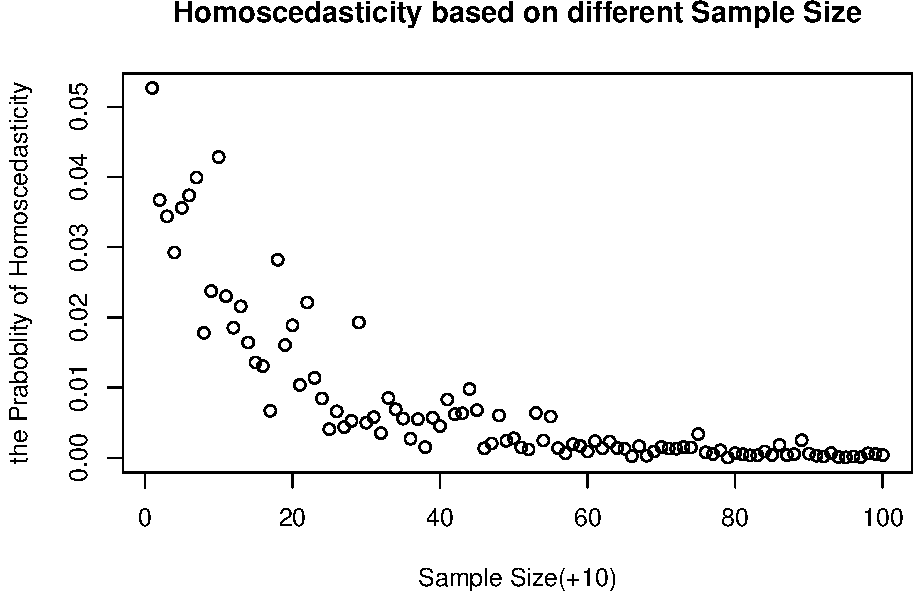
\includegraphics{BST169Coursework_project_answer_files/figure-latex/Monte Carlo:heter-uncorrected-1.pdf}

\begin{Shaded}
\begin{Highlighting}[]
\CommentTok{#plot(P.value_W_chisq_container/(loop*10), xlab = "Sample Size(+10)",ylab = "the P-value of Wald statistcs following the chisq distribution",main="Homoscedasticity based on different Sample Size")}
\CommentTok{#plot(P.value_LM_chisq_container/(loop*10),xlab = "Sample Size(+10)",ylab = "the P-value of LM statistcs following the chisq distribution(under 5%)",main="the P-value of LM~chisq based on different Sample Size")}
\KeywordTok{par}\NormalTok{(}\DataTypeTok{mfrow=}\KeywordTok{c}\NormalTok{(}\DecValTok{3}\NormalTok{,}\DecValTok{1}\NormalTok{))}
\KeywordTok{plot}\NormalTok{(W_count/(loop),}\DataTypeTok{xlab =} \StringTok{"Sample Size(+10)"}\NormalTok{,}\DataTypeTok{ylab =} \StringTok{"the Praboblity of Wald statistcs following the chisq distribution(under 5%)"}\NormalTok{,}\DataTypeTok{main=}\StringTok{"the Praboblity of Wald~chisq based on different Sample Size"}\NormalTok{)}
\KeywordTok{points}\NormalTok{(}\KeywordTok{lowess}\NormalTok{(W_count/(loop)),}\DataTypeTok{type=}\StringTok{"l"}\NormalTok{,}\DataTypeTok{col=}\StringTok{"red"}\NormalTok{)}
\KeywordTok{plot}\NormalTok{(LM_count/(loop),}\DataTypeTok{xlab =} \StringTok{"Sample Size(+10)"}\NormalTok{,}\DataTypeTok{ylab =} \StringTok{"the Praboblity of LM statistcs following the chisq distribution(under 5%)"}\NormalTok{,}\DataTypeTok{main=}\StringTok{"the Praboblity of LM~chisq based on different Sample Size"}\NormalTok{)}
\KeywordTok{points}\NormalTok{(}\KeywordTok{lowess}\NormalTok{(LM_count/(loop)),}\DataTypeTok{type=}\StringTok{"l"}\NormalTok{,}\DataTypeTok{col=}\StringTok{"red"}\NormalTok{)}
\KeywordTok{plot}\NormalTok{(LR_count/(loop),}\DataTypeTok{xlab =} \StringTok{"Sample Size(+10)"}\NormalTok{,}\DataTypeTok{ylab =} \StringTok{"the Praboblity of LR statistcs following the chisq distribution(under 5%)"}\NormalTok{,}\DataTypeTok{main=}\StringTok{"the Praboblity of LR~chisq based on different Sample Size"}\NormalTok{)}
\KeywordTok{points}\NormalTok{(}\KeywordTok{lowess}\NormalTok{(LR_count/(loop)),}\DataTypeTok{type=}\StringTok{"l"}\NormalTok{,}\DataTypeTok{col=}\StringTok{"red"}\NormalTok{)}
\end{Highlighting}
\end{Shaded}

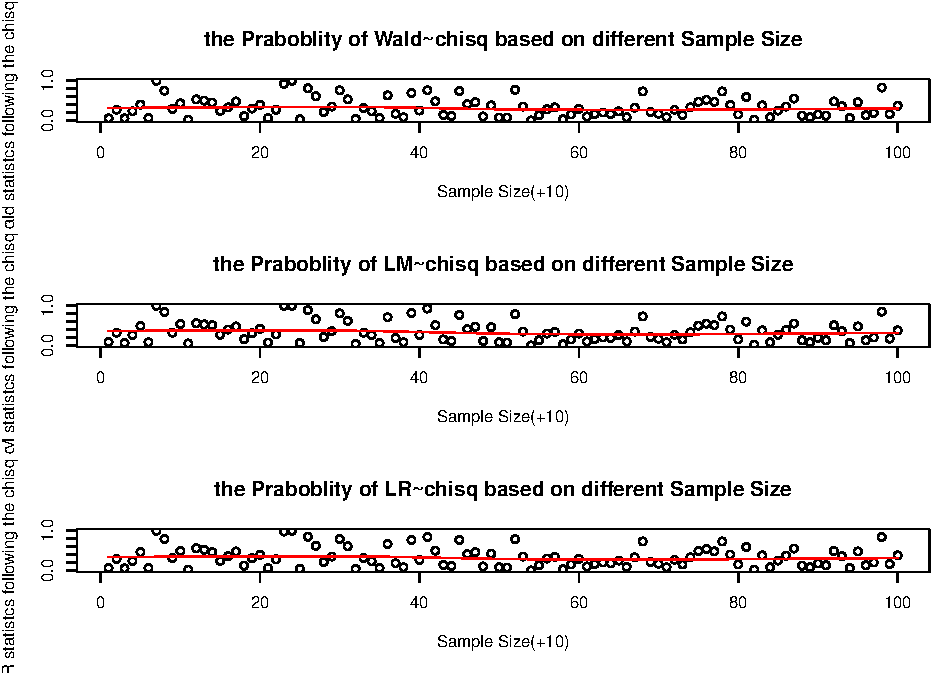
\includegraphics{BST169Coursework_project_answer_files/figure-latex/Monte Carlo:heter-uncorrected-2.pdf}
From Homoscedasticity plot , I can find when the size of sample
increases, the probablity of the Homoscedasticity of equ1 will decrease.

Thus, there exist the heteroscedacity issue to make the Wald and LM test
invalid.

From these Praboblity of Wald\textsubscript{chisq/LM}chisq plots, I can
find the distribution of p-value of ks.test of each statistcs. And they
both own decreasing trend depend on sample size. and more importantly,
the p-value of Wald and LM statistics are almost less than the 5\% of
signiifcant level, which means the Wald and LM statistics are invalid.
Thus, I should correct the model.

I choose WLS to elimate the heteroscedacity. However, I should seek a
appropriate weigths to procedure the WLS. normally choose the Inverse of
independent variable with m power as weights. But here, i choose
\(1/sqrt(x1)\)

\begin{Shaded}
\begin{Highlighting}[]
\KeywordTok{require}\NormalTok{(lmtest)}
\KeywordTok{require}\NormalTok{(MASS)}


\NormalTok{##boost up: translate programme language code into Byte-code.}
\KeywordTok{require}\NormalTok{(compiler)}
\KeywordTok{enableJIT}\NormalTok{(}\DecValTok{3}\NormalTok{)}
\end{Highlighting}
\end{Shaded}

\begin{verbatim}
## [1] 3
\end{verbatim}

\begin{Shaded}
\begin{Highlighting}[]
\NormalTok{##boost up-end for continues}
\CommentTok{#set seed}
\KeywordTok{set.seed}\NormalTok{(}\DecValTok{2112}\NormalTok{)}
\CommentTok{#assumption part}

\NormalTok{loop=}\DecValTok{100}
\NormalTok{m=}\DecValTok{1}\CommentTok{#I have a multiplication factor:1, which means when you set loop=N, }
\CommentTok{#It will generate N different (increased) sample size, and for each sample will do N*10 times Monte Carlo simulations.}
\CommentTok{#be careful your settings, your computer may explode.}
\CommentTok{#Warning: the loop time cannot be larger any more;please forgive me, this all my Macbook fault. And the optimization of R is terrible.}

\NormalTok{beta_1=}\FloatTok{0.4}
\NormalTok{beta_0=}\DecValTok{1}

\CommentTok{#x1_store=rchisq(80+20, 2)}
\CommentTok{#initial valueset}
\NormalTok{original_N=}\DecValTok{30}
\NormalTok{signlevel=}\FloatTok{0.05}

\CommentTok{#initial container for Wald, LM, LR}
\NormalTok{W_count=}\KeywordTok{rep}\NormalTok{(}\DecValTok{0}\NormalTok{,loop)}
\NormalTok{LM_count=}\KeywordTok{rep}\NormalTok{(}\DecValTok{0}\NormalTok{,loop)}
\NormalTok{LR_count=}\KeywordTok{rep}\NormalTok{(}\DecValTok{0}\NormalTok{,loop)}
\NormalTok{P.value_homo_container=}\KeywordTok{rep}\NormalTok{(}\DecValTok{0}\NormalTok{,loop)}
\NormalTok{P.value_W_chisq_container=}\KeywordTok{rep}\NormalTok{(}\DecValTok{0}\NormalTok{,loop)}
\NormalTok{P.value_LM_chisq_container=}\KeywordTok{rep}\NormalTok{(}\DecValTok{0}\NormalTok{,loop)}

\CommentTok{# for loop start:Monte Carlo}

\NormalTok{for(j in }\DecValTok{1}\NormalTok{:loop)\{}\CommentTok{#first for-loop for generating multi-sample}
\NormalTok{W=}\DecValTok{0}
\NormalTok{LM=}\DecValTok{0}
\NormalTok{LR=}\DecValTok{0}
\NormalTok{N=original_N+j}

\CommentTok{#generation part:data}
\NormalTok{x1=}\KeywordTok{rchisq}\NormalTok{(N, }\DecValTok{2}\NormalTok{)}
\NormalTok{x2=}\KeywordTok{runif}\NormalTok{(N,}\DecValTok{0}\NormalTok{,}\DecValTok{10}\NormalTok{)}

\NormalTok{for (i in }\DecValTok{1}\NormalTok{:loop*m)\{}\CommentTok{# second for-loop: the main Monte Carlo code}
\NormalTok{e=}\KeywordTok{rt}\NormalTok{(N,}\DecValTok{6}\NormalTok{)}
\NormalTok{U_q=}\KeywordTok{matrix}\NormalTok{(}\DecValTok{0}\NormalTok{,}\DecValTok{3}\NormalTok{,}\DecValTok{3}\NormalTok{)}
\NormalTok{U_tilde=}\KeywordTok{matrix}\NormalTok{(}\DecValTok{0}\NormalTok{,}\DecValTok{3}\NormalTok{,}\DecValTok{3}\NormalTok{)}
\NormalTok{R=}\KeywordTok{cbind}\NormalTok{(}\DecValTok{0}\NormalTok{,}\DecValTok{1}\NormalTok{,}\DecValTok{1}\NormalTok{)}
\NormalTok{r=}\KeywordTok{cbind}\NormalTok{(}\DecValTok{1}\NormalTok{,}\DecValTok{0}\NormalTok{,}\DecValTok{0}\NormalTok{)}
\NormalTok{X=}\KeywordTok{cbind}\NormalTok{(}\KeywordTok{rep}\NormalTok{(}\DecValTok{1}\NormalTok{,N),x1,x2)}
\NormalTok{y=beta_0+beta_1*x1+(}\DecValTok{1}\NormalTok{-beta_1)*x2+}\KeywordTok{sqrt}\NormalTok{(x1)*e}
\CommentTok{#generation part:regression}
\NormalTok{equ1<-}\KeywordTok{lm}\NormalTok{(y~x1+x2,}\DataTypeTok{weights=}\DecValTok{1}\NormalTok{/(x1^.}\DecValTok{5}\NormalTok{))}
\NormalTok{equ2<-}\KeywordTok{lm}\NormalTok{(}\KeywordTok{I}\NormalTok{(y-x2)~}\KeywordTok{I}\NormalTok{(x1-x2),}\DataTypeTok{weights=}\DecValTok{1}\NormalTok{/(x1^.}\DecValTok{5}\NormalTok{))}
\CommentTok{#heter}
\NormalTok{if (}\KeywordTok{bptest}\NormalTok{(}\KeywordTok{resid}\NormalTok{(equ1)^}\DecValTok{2}\NormalTok{~x1*x2+x1^}\DecValTok{2}\NormalTok{+x2^}\DecValTok{2}\NormalTok{)$p.value<signlevel)\{}
\NormalTok{equ1<-}\KeywordTok{lm}\NormalTok{(y~x1+x2,}\DataTypeTok{weights=}\DecValTok{1}\NormalTok{/}\KeywordTok{sqrt}\NormalTok{(x1))}
\NormalTok{equ2<-}\KeywordTok{lm}\NormalTok{(}\KeywordTok{I}\NormalTok{(y-x2)~}\KeywordTok{I}\NormalTok{(x1-x2),}\DataTypeTok{weights=}\DecValTok{1}\NormalTok{/}\KeywordTok{sqrt}\NormalTok{(x1))}
\NormalTok{\}}
\CommentTok{#calculate beta and residual}
\NormalTok{beta=}\KeywordTok{matrix}\NormalTok{(equ1$coefficients)}
\NormalTok{residual=}\KeywordTok{matrix}\NormalTok{(}\KeywordTok{resid}\NormalTok{(equ1))}
\CommentTok{#calc SSR and Wald,LM, and LR}
\CommentTok{#U_N}
\CommentTok{#}
\NormalTok{for(i in }\DecValTok{1}\NormalTok{:N)\{U_tilde=U_tilde+residual[i,]^}\DecValTok{2}\NormalTok{*X[i,]%*%}\KeywordTok{t}\NormalTok{(X[i,])\}}
\NormalTok{U_tilde=U_tilde/N}
\CommentTok{#U_q}
\NormalTok{est_y=equ2$coefficients[}\DecValTok{1}\NormalTok{]+equ2$coefficients[}\DecValTok{2}\NormalTok{]*(x1-x2)+}\KeywordTok{sqrt}\NormalTok{(x1)*e+x2}
\NormalTok{temp_y=}\KeywordTok{matrix}\NormalTok{(est_y-}\KeywordTok{mean}\NormalTok{(est_y))}
\NormalTok{for(i in }\DecValTok{1}\NormalTok{:N)\{U_q=U_q+temp_y[i,]^}\DecValTok{2}\NormalTok{*X[i,]%*%}\KeywordTok{t}\NormalTok{(X[i,])\}}
\NormalTok{U_q=U_q/N}
\CommentTok{#calculate Wald and LM}
\NormalTok{W[j]=(}\DecValTok{1}\NormalTok{/N)*}\KeywordTok{t}\NormalTok{(R%*%beta}\DecValTok{-1}\NormalTok{)%*%}\KeywordTok{solve}\NormalTok{(R%*%}\KeywordTok{solve}\NormalTok{(}\KeywordTok{t}\NormalTok{(X)%*%X)%*%U_tilde%*%}\KeywordTok{solve}\NormalTok{(}\KeywordTok{t}\NormalTok{(X)%*%X)%*%}\KeywordTok{t}\NormalTok{(R))%*%(R%*%beta}\DecValTok{-1}\NormalTok{)}
\NormalTok{LM[j]=(}\DecValTok{1}\NormalTok{/N)*}\KeywordTok{t}\NormalTok{(R%*%beta}\DecValTok{-1}\NormalTok{)%*%}\KeywordTok{solve}\NormalTok{(R%*%}\KeywordTok{solve}\NormalTok{(}\KeywordTok{t}\NormalTok{(X)%*%X)%*%U_q%*%}\KeywordTok{solve}\NormalTok{(}\KeywordTok{t}\NormalTok{(X)%*%X)%*%}\KeywordTok{t}\NormalTok{(R))%*%(R%*%beta}\DecValTok{-1}\NormalTok{)}
\CommentTok{#SSRu=sum(residuals(equ1)^2)}
\CommentTok{#SSRr=sum(residuals(equ2)^2)}

\CommentTok{#W[i]=N*((SSRr-SSRu)/(SSRu))}
\CommentTok{#LM[i]=N*((SSRr-SSRu)/(SSRr))}
\CommentTok{#LR[i]=N*(log(SSRr/SSRu))}


\CommentTok{#if (bptest(equ1,studentize = 0)$p.value<signlevel)\{P.value_homo_container[j]=P.value_homo_container[j]+1\}}
\NormalTok{P.value_homo_container[j]=P.value_homo_container[j]+}\KeywordTok{bptest}\NormalTok{(equ1,}\DataTypeTok{studentize =} \DecValTok{0}\NormalTok{)$p.value}
\NormalTok{P.value_W_chisq_container[j]=P.value_W_chisq_container[j]+}\KeywordTok{ks.test}\NormalTok{(W,}\StringTok{'pchisq'}\NormalTok{,}\DecValTok{1}\NormalTok{)$p.value}
\NormalTok{P.value_LM_chisq_container[j]=P.value_LM_chisq_container[j]+}\KeywordTok{ks.test}\NormalTok{(LM,}\StringTok{'pchisq'}\NormalTok{,}\DecValTok{1}\NormalTok{)$p.value}
\NormalTok{if(}\KeywordTok{ks.test}\NormalTok{(W,}\StringTok{'pchisq'}\NormalTok{,}\DecValTok{1}\NormalTok{)$p.value>signlevel)\{W_count[j]=W_count[j]+}\DecValTok{1}\NormalTok{\}}
\NormalTok{if(}\KeywordTok{ks.test}\NormalTok{(LM,}\StringTok{'pchisq'}\NormalTok{,}\DecValTok{1}\NormalTok{)$p.value>signlevel)\{LM_count[j]=LM_count[j]+}\DecValTok{1}\NormalTok{\}}
\CommentTok{#if(ks.test(LR,'pchisq',1)$p.value>signlevel)\{LR_count[j]=LR_count[j]+1\}}
\KeywordTok{gc}\NormalTok{()}
\NormalTok{\}}

\NormalTok{\}}

\CommentTok{#plot(P.value_homo_container/(loop*m), xlab = "Sample Size(+10)",ylab = "the P-value of Homoscedasticity",main="Homoscedasticity based on different Sample Size")}
\CommentTok{#plot(P.value_W_chisq_container/(loop*m), xlab = "Sample Size(+10)",ylab = "the P-value of Wald statistcs following the chisq distribution",main="Homoscedasticity based on different Sample Size")}
\CommentTok{#plot(P.value_LM_chisq_container/(loop*m),xlab = "Sample Size(+10)",ylab = "the P-value of LM statistcs following the chisq distribution(under 5%)",main="the P-value of LM~chisq based on different Sample Size")}
\KeywordTok{par}\NormalTok{(}\DataTypeTok{mfrow=}\KeywordTok{c}\NormalTok{(}\DecValTok{2}\NormalTok{,}\DecValTok{1}\NormalTok{))}
\KeywordTok{plot}\NormalTok{(W_count/(loop*m),}\DataTypeTok{xlab =} \StringTok{"Sample Size(+30)"}\NormalTok{,}\DataTypeTok{ylab =} \StringTok{"the Praboblity of Wald statistcs following the chisq distribution(under 5%)"}\NormalTok{,}\DataTypeTok{main=}\StringTok{"the Praboblity of Wald~chisq based on different Sample Size"}\NormalTok{)}
\KeywordTok{points}\NormalTok{(}\KeywordTok{lowess}\NormalTok{(W_count/(loop*m)),}\DataTypeTok{type=}\StringTok{"l"}\NormalTok{,}\DataTypeTok{col=}\StringTok{"red"}\NormalTok{)}
\KeywordTok{plot}\NormalTok{(LM_count/(loop*m),}\DataTypeTok{xlab =} \StringTok{"Sample Size(+30)"}\NormalTok{,}\DataTypeTok{ylab =} \StringTok{"the Praboblity of LM statistcs following the chisq distribution(under 5%)"}\NormalTok{,}\DataTypeTok{main=}\StringTok{"the Praboblity of LM~chisq based on different Sample Size"}\NormalTok{)}
\KeywordTok{points}\NormalTok{(}\KeywordTok{lowess}\NormalTok{(LM_count/(loop*m)),}\DataTypeTok{type=}\StringTok{"l"}\NormalTok{,}\DataTypeTok{col=}\StringTok{"red"}\NormalTok{)}
\end{Highlighting}
\end{Shaded}

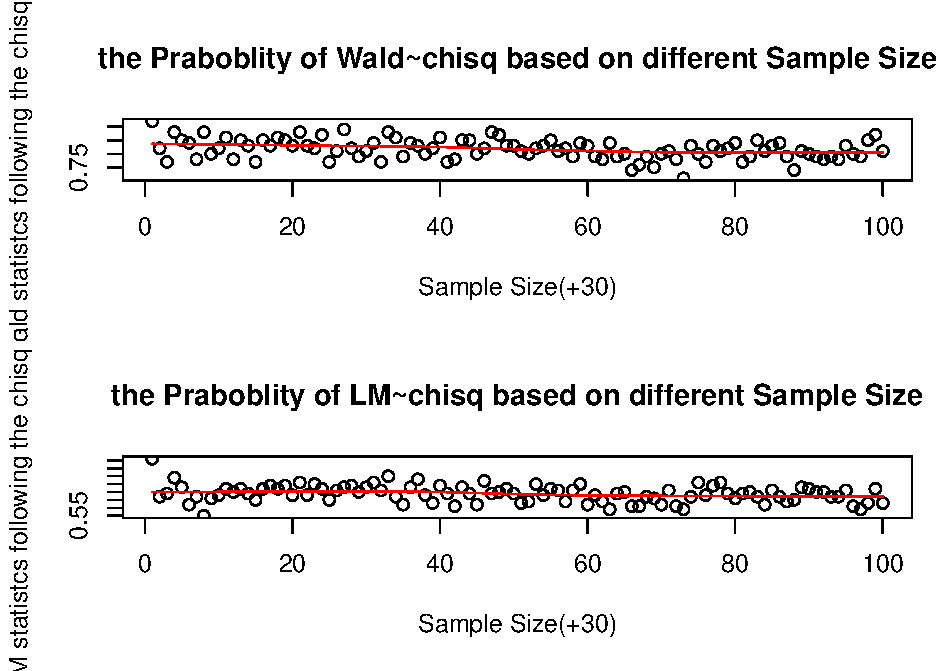
\includegraphics{BST169Coursework_project_answer_files/figure-latex/Monte Carlo:heter-corrected-1.pdf}

\begin{Shaded}
\begin{Highlighting}[]
\CommentTok{#plot(LR_count/(loop*m),xlab = "Sample Size(+30)",ylab = "the Praboblity of LR statistcs following the chisq distribution(under 5%)",main="the Praboblity of LR~chisq based on different Sample Size")}
\end{Highlighting}
\end{Shaded}

From these plots, after corrected heteroscedacity issue, I can find that
the Wald and LM statistics are valid, all the p-value of ks.test of each
test statistics are over 5\%, which means the these test statistics
follow the chi-squared distribution.that is consistent with the
definition of their own.

\subsection{Question 4}\label{question-4}

Compare the size of different test statistics (frequencies of making
Type 1 error) from Monte Carlo using 5\% level of significance for
different sample sizes. Explain the results.

\begin{Shaded}
\begin{Highlighting}[]
\KeywordTok{require}\NormalTok{(lmtest)}
\KeywordTok{require}\NormalTok{(MASS)}


\NormalTok{##boost up: translate programme language code into Byte-code.}
\KeywordTok{require}\NormalTok{(compiler)}
\KeywordTok{enableJIT}\NormalTok{(}\DecValTok{3}\NormalTok{)}
\end{Highlighting}
\end{Shaded}

\begin{verbatim}
## [1] 3
\end{verbatim}

\begin{Shaded}
\begin{Highlighting}[]
\NormalTok{##boost up-end for continues}
\CommentTok{#set seed}
\KeywordTok{set.seed}\NormalTok{(}\DecValTok{2112}\NormalTok{)}
\CommentTok{#assumption part}

\NormalTok{loop=}\DecValTok{100}
\NormalTok{m=}\DecValTok{1}\CommentTok{#I have a multiplication factor:1, which means when you set loop=N, }
\CommentTok{#It will generate N different (increased) sample size, and for each sample will do N*10 times Monte Carlo simulations.}
\CommentTok{#be careful your settings, your computer may explode.}
\CommentTok{#Warning: the loop time cannot be larger any more;please forgive me, this all my Macbook fault. And the optimization of R is terrible.}

\NormalTok{beta_1=}\FloatTok{0.4}
\NormalTok{beta_0=}\DecValTok{1}

\CommentTok{#x1_store=rchisq(80+20, 2)}
\CommentTok{#initial valueset}
\NormalTok{original_N=}\DecValTok{10}
\NormalTok{signlevel=}\FloatTok{0.05}

\CommentTok{#initial container for Wald, LM, LR}
\NormalTok{W=}\KeywordTok{rep}\NormalTok{(}\DecValTok{0}\NormalTok{,loop)}
\NormalTok{LM=}\KeywordTok{rep}\NormalTok{(}\DecValTok{0}\NormalTok{,loop)}
\NormalTok{LR=}\KeywordTok{rep}\NormalTok{(}\DecValTok{0}\NormalTok{,loop)}
\NormalTok{W_count=}\KeywordTok{rep}\NormalTok{(}\DecValTok{0}\NormalTok{,loop)}
\NormalTok{LM_count=}\KeywordTok{rep}\NormalTok{(}\DecValTok{0}\NormalTok{,loop)}
\NormalTok{LR_count=}\KeywordTok{rep}\NormalTok{(}\DecValTok{0}\NormalTok{,loop)}
\NormalTok{P.value_homo_container=}\KeywordTok{rep}\NormalTok{(}\DecValTok{0}\NormalTok{,loop)}
\NormalTok{P.value_W_chisq_container=}\KeywordTok{rep}\NormalTok{(}\DecValTok{0}\NormalTok{,loop)}
\NormalTok{P.value_LM_chisq_container=}\KeywordTok{rep}\NormalTok{(}\DecValTok{0}\NormalTok{,loop)}
\NormalTok{theta=}\KeywordTok{rep}\NormalTok{(}\KeywordTok{seq}\NormalTok{(}\FloatTok{0.25}\NormalTok{,}\FloatTok{1.75}\NormalTok{,}\DataTypeTok{len=}\NormalTok{loop))}
\NormalTok{crv=}\KeywordTok{rep}\NormalTok{(}\KeywordTok{qchisq}\NormalTok{(}\FloatTok{0.95}\NormalTok{,}\DecValTok{1}\NormalTok{),loop)}





\CommentTok{# for loop start:Monte Carlo}
\CommentTok{#for(j in 1:loop)\{#first for-loop for generating multi-sample}



\CommentTok{#generation part:data}


\CommentTok{#U_q=matrix(0,3,3)}
\CommentTok{#U_tilde=matrix(0,3,3)}
\CommentTok{#R=cbind(0,1,1)}
\CommentTok{#r=cbind(1,0,0)}
\CommentTok{#X=cbind(rep(1,N),x1,x2)}

\NormalTok{for(j in }\DecValTok{1}\NormalTok{:loop)\{}
\NormalTok{N=original_N+j}
\NormalTok{x1=}\KeywordTok{rchisq}\NormalTok{(N, }\DecValTok{2}\NormalTok{)}
\NormalTok{x2=}\KeywordTok{runif}\NormalTok{(N,}\DecValTok{0}\NormalTok{,}\DecValTok{10}\NormalTok{)}

\NormalTok{for (i in }\DecValTok{1}\NormalTok{:loop*m)\{}\CommentTok{# second for-loop: the main Monte Carlo code}
\NormalTok{e=}\KeywordTok{rnorm}\NormalTok{(N,}\DecValTok{0}\NormalTok{,}\DecValTok{1}\NormalTok{)}
\NormalTok{y=beta_0+beta_1*x1+(}\DecValTok{1}\NormalTok{-beta_1)*x2+}\KeywordTok{sqrt}\NormalTok{(x1)*e}
\CommentTok{#generation part:regression}
\CommentTok{#true_equ2<-lm(I(y-x2)~I(x1-x2),weights=1/sqrt(x1))}
\NormalTok{equ1<-}\KeywordTok{lm}\NormalTok{(y~x1+x2,}\DataTypeTok{weights=}\DecValTok{1}\NormalTok{/}\KeywordTok{sqrt}\NormalTok{(x1))}
\NormalTok{equ2<-}\KeywordTok{lm}\NormalTok{(}\KeywordTok{I}\NormalTok{(y-theta[i]*x2)~}\KeywordTok{I}\NormalTok{(x1-x2),}\DataTypeTok{weights=}\DecValTok{1}\NormalTok{/}\KeywordTok{sqrt}\NormalTok{(x1))}

\NormalTok{SSRu=}\KeywordTok{sum}\NormalTok{(}\KeywordTok{residuals}\NormalTok{(equ1)^}\DecValTok{2}\NormalTok{)}
\NormalTok{SSRr=}\KeywordTok{sum}\NormalTok{(}\KeywordTok{residuals}\NormalTok{(equ2)^}\DecValTok{2}\NormalTok{)}
\CommentTok{#true_SSRr=sum(residuals(true_equ2)^2)}
\NormalTok{W[i]=W[i]+N*((SSRr-SSRu)/(SSRu))}
\NormalTok{LM[i]=LM[i]+N*((SSRr-SSRu)/(SSRr))}
\NormalTok{LR[i]=LR[i]+N*(}\KeywordTok{log}\NormalTok{(SSRr/SSRu))}

\CommentTok{#LR[i]=N*(log(SSRr/SSRu))}
\NormalTok{W_count[j]=W_count[j]+(}\KeywordTok{mean}\NormalTok{(W)>}\KeywordTok{qchisq}\NormalTok{(}\FloatTok{0.95}\NormalTok{,}\DecValTok{1}\NormalTok{))}
\NormalTok{LM_count[j]=LM_count[j]+(}\KeywordTok{mean}\NormalTok{(LM)>}\KeywordTok{qchisq}\NormalTok{(}\FloatTok{0.95}\NormalTok{,}\DecValTok{1}\NormalTok{))}
\NormalTok{LR_count[j]=LR_count[j]+(}\KeywordTok{mean}\NormalTok{(LR)>}\KeywordTok{qchisq}\NormalTok{(}\FloatTok{0.95}\NormalTok{,}\DecValTok{1}\NormalTok{))}
\NormalTok{\}}

\NormalTok{\}}
\CommentTok{#W_count=W_count+(ks.test(W,'pchisq',1)$p.value>signlevel)}
\CommentTok{#LM_count=LM_count+(ks.test(LM,'pchisq',1)$p.value>signlevel)}
\KeywordTok{par}\NormalTok{(}\DataTypeTok{mfrow=}\KeywordTok{c}\NormalTok{(}\DecValTok{3}\NormalTok{,}\DecValTok{1}\NormalTok{))}
\KeywordTok{plot}\NormalTok{(W/(loop*m),}\DataTypeTok{xlab =} \StringTok{"Sample Size(+10)"}\NormalTok{,}\DataTypeTok{ylab =} \StringTok{"the Wald statistcs(under 5%)"}\NormalTok{,}\DataTypeTok{main=}\StringTok{"the Wald staitsices based on different Sample Size"}\NormalTok{)}
\KeywordTok{points}\NormalTok{(crv,}\DataTypeTok{type=}\StringTok{"l"}\NormalTok{,}\DataTypeTok{col=}\StringTok{"red"}\NormalTok{)}

\KeywordTok{plot}\NormalTok{(LM/(loop*m),}\DataTypeTok{xlab =} \StringTok{"Sample Size(+10)"}\NormalTok{,}\DataTypeTok{ylab =} \StringTok{"the LM statistcs(under 5%)"}\NormalTok{,}\DataTypeTok{main=}\StringTok{"the Praboblity of LM~chisq based on different Sample Size"}\NormalTok{)}
\CommentTok{#points(lowess(LM/(loop*m)),type="l",col="red")}
\KeywordTok{points}\NormalTok{(crv,}\DataTypeTok{type=}\StringTok{"l"}\NormalTok{,}\DataTypeTok{col=}\StringTok{"red"}\NormalTok{)}
\KeywordTok{plot}\NormalTok{(LR/(loop*m),}\DataTypeTok{xlab =} \StringTok{"Sample Size(+10)"}\NormalTok{,}\DataTypeTok{ylab =} \StringTok{"the LR statistcs(under 5%)"}\NormalTok{,}\DataTypeTok{main=}\StringTok{"the LR based on different Sample Size"}\NormalTok{)}
\KeywordTok{points}\NormalTok{(crv,}\DataTypeTok{type=}\StringTok{"l"}\NormalTok{,}\DataTypeTok{col=}\StringTok{"red"}\NormalTok{)}
\end{Highlighting}
\end{Shaded}

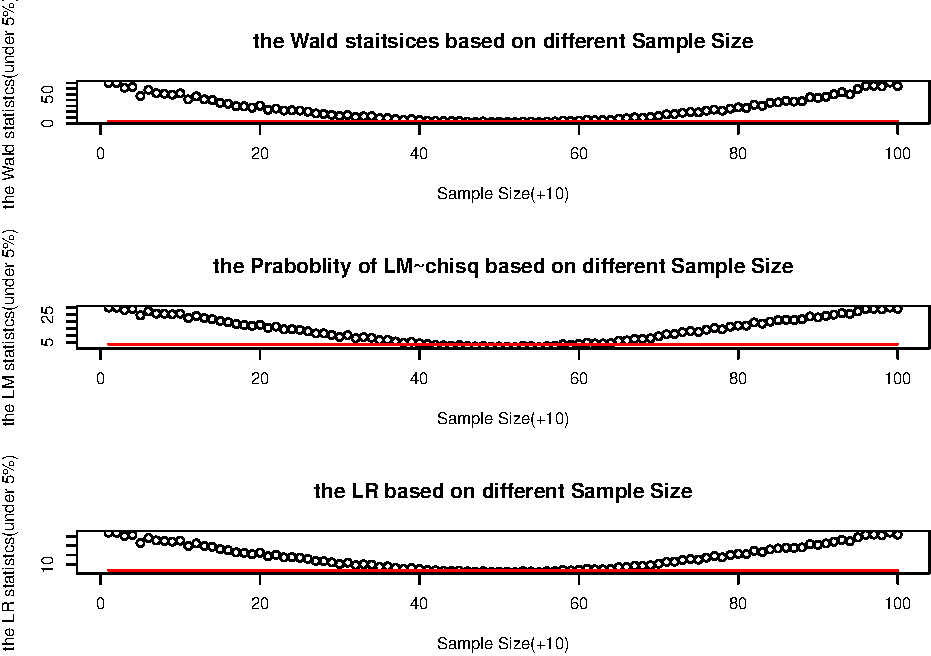
\includegraphics{BST169Coursework_project_answer_files/figure-latex/Monte Carlo:type1error-1.pdf}

\begin{Shaded}
\begin{Highlighting}[]
\CommentTok{#plot(W_count/(loop*m),xlab = "Sample Size(+10)",ylab = "the Wald statistcs following the chisq distribution(under 5%)",main="the Wald staitsices based on different Sample Size")}
\CommentTok{#points(crv,type="l",col="red")}

\CommentTok{#plot(LM/(loop*m),xlab = "Sample Size(+10)",ylab = "the LM statistcs following the chisq distribution(under 5%)",main="the Praboblity of LM~chisq based on different Sample Size")}
\CommentTok{#points(lowess(LM/(loop*m)),type="l",col="red")}
\CommentTok{#points(crv,type="l",col="red")}
\CommentTok{#plot(LR/(loop*m),xlab = "Sample Size(+10)",ylab = "the LR statistcs following the chisq distribution(under 5%)",main="the Praboblity of LR~chisq based on different Sample Size")}
\CommentTok{#points(crv,type="l",col="red")}
\end{Highlighting}
\end{Shaded}

from these test statistics plots, I can find that after sample size=50,
the wald, LM and LR statistcs will increase by the sample size. And
before 50, will decrease by the sample size.

I aslo do the t test for \(\beta_{1} + \beta_{2} = 1\) to show the type
I error.

\begin{Shaded}
\begin{Highlighting}[]
\KeywordTok{require}\NormalTok{(lmtest)}
\KeywordTok{require}\NormalTok{(MASS)}

\NormalTok{##boost up: translate programme language code into Byte-code.}
\KeywordTok{require}\NormalTok{(compiler)}
\KeywordTok{enableJIT}\NormalTok{(}\DecValTok{3}\NormalTok{)}
\end{Highlighting}
\end{Shaded}

\begin{verbatim}
## [1] 3
\end{verbatim}

\begin{Shaded}
\begin{Highlighting}[]
\NormalTok{##boost up-end for continues}
\CommentTok{#assumption part}

\NormalTok{loop=}\DecValTok{100}
\CommentTok{#Warning: the loop time cannot be larger any more;please forgive me, this all my Macbook fault. And the optimization of R is terrible.}
\CommentTok{#initial valueset}
\NormalTok{original_N=}\DecValTok{100}
\NormalTok{signlevel=}\FloatTok{0.05}
\NormalTok{theta_count=}\KeywordTok{rep}\NormalTok{(}\DecValTok{0}\NormalTok{,loop)}
\CommentTok{# for loop start:Monte Carlo}
\NormalTok{for(j in }\DecValTok{1}\NormalTok{:loop)\{}\CommentTok{#first for-loop for generating multi-sample}
\NormalTok{theta=}\DecValTok{0}
\NormalTok{N=original_N+j}
\CommentTok{#generation part:data}
\NormalTok{s=}\KeywordTok{sample}\NormalTok{(}\DecValTok{1}\NormalTok{:}\KeywordTok{length}\NormalTok{(pbp$y),N,}\DataTypeTok{replace =} \DecValTok{1}\NormalTok{)}
\NormalTok{question.pre.y<-pbp$y[s]}
\NormalTok{question.pre.x1<-pbp$x1[s]}
\NormalTok{question.pre.x2<-pbp$x2[s]}
\NormalTok{pre_equ<-}\KeywordTok{lm}\NormalTok{(}\KeywordTok{I}\NormalTok{(question.pre.y-question.pre.x2)~}\KeywordTok{I}\NormalTok{(question.pre.x1-question.pre.x2))}
\NormalTok{theta_test=}\KeywordTok{rep}\NormalTok{(}\KeywordTok{seq}\NormalTok{(}\DecValTok{0}\NormalTok{,}\DecValTok{4}\NormalTok{,}\DataTypeTok{len=}\NormalTok{loop))}
\NormalTok{for (i in }\DecValTok{1}\NormalTok{:loop*}\DecValTok{10}\NormalTok{)\{}
\NormalTok{question5.residuals=}\KeywordTok{sample}\NormalTok{(}\KeywordTok{residuals}\NormalTok{(pre_equ),N,}\DataTypeTok{replace=}\DecValTok{1}\NormalTok{)}
\NormalTok{question5.y=pre_equ$coefficients[}\DecValTok{1}\NormalTok{]+pre_equ$coefficients[}\DecValTok{2}\NormalTok{]*question.pre.x1+(}\DecValTok{1}\NormalTok{-pre_equ$coefficients[}\DecValTok{2}\NormalTok{])*question.pre.x2+question5.residuals}
\CommentTok{#generation part:regression}
\NormalTok{question5.equ1<-}\KeywordTok{lm}\NormalTok{(question5.y~question.pre.x1+question.pre.x2)}
\CommentTok{#residuals.question5.equ1=resid(question5.equ1)}
\CommentTok{#question5.equ1<-lm((question5.y-question5.x2)~(question5.x1-question5.x2))}
\CommentTok{#calculation}
\NormalTok{##pre-cal:heteroscedasticity}
\CommentTok{#if(bptest(residuals.question5.equ1^2~question5.x1*question5.x2+question5.x1^2+question5.x2^2)$p.value<signlevel)\{}
\CommentTok{#  question5.equ1<-lm(question5.y~question5.x1+question5.x2,weights=(1/question5.x1^0.5))}
  \CommentTok{#question5.equ1<-lm((question5.y-question5.x2)~(question5.x1-question5.x2),weights=(1/question5.x1^0.5))\}}
\CommentTok{#calc }
\NormalTok{theta[i]=question5.equ1$coefficients[}\DecValTok{2}\NormalTok{]+question5.equ1$coefficients[}\DecValTok{3}\NormalTok{]}
\CommentTok{#if(length(theta)>2)\{if(t.test(theta,mu=1)$p.value>signlevel)\{theta_count[j]=theta_count[j]+1\}\}}
\NormalTok{theta_count[j]=theta_count[j]+(}\KeywordTok{t.test}\NormalTok{(theta,}\DataTypeTok{mu=}\NormalTok{theta_test[j])$p.value<}\FloatTok{0.05}\NormalTok{)}
\NormalTok{\}}
\NormalTok{\}}


\KeywordTok{plot}\NormalTok{(theta_test,theta_count/(loop*}\DecValTok{10}\NormalTok{),}\DataTypeTok{xlab=}\StringTok{"Theta(beta1+beta2)"}\NormalTok{,}\DataTypeTok{ylab=}\StringTok{"Praboblity of Type 1 error"}\NormalTok{,}\DataTypeTok{main=}\StringTok{"The Praboblity of Type 1 error"}\NormalTok{)}
\end{Highlighting}
\end{Shaded}

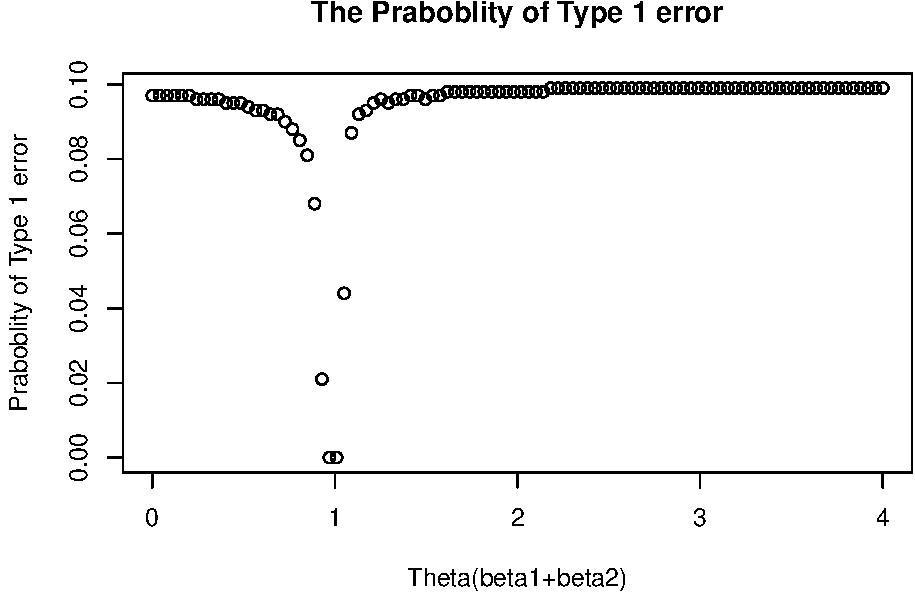
\includegraphics{BST169Coursework_project_answer_files/figure-latex/Monte Carlo for type1error-1.pdf}

form graph, I can find that the Theta which equals to
\(\beta_1+\beta_2=1\), when the type I error will dramatically increase
when theta has a value different from true 1.

\subsection{Question 5}\label{question-5}

For the data set pbp.csv, suppose Equation (2) is the true model. Use
proper bootstrapped errors from the true model to study whether
different test statistics for H0 : \(\beta_{1} + \beta_{2} = 1\) in the
previous questions follow chi-squared distribution. Explain your
results.

\begin{Shaded}
\begin{Highlighting}[]
\NormalTok{pbp=}\KeywordTok{read.csv}\NormalTok{(}\StringTok{"/Users/sn0wfree/Dropbox/PhD_1st_study/BST169_Econometrics/Crousework_Project/pbp.csv"}\NormalTok{)}
\NormalTok{loop=}\DecValTok{50}
\NormalTok{m=}\DecValTok{1}\CommentTok{#I have a multiplication factor:1, which means when you set loop=N, }
\CommentTok{#It will generate N different (increased) sample size, and for each sample will do N*10 times Monte Carlo simulations.}
\CommentTok{#be careful your settings, your computer may explode.}
\CommentTok{#Warning: the loop time cannot be larger any more;please forgive me, this all my Macbook fault. And the optimization of R is terrible.}


\CommentTok{#initial valueset}
\NormalTok{original_N=}\DecValTok{30}
\NormalTok{signlevel=}\FloatTok{0.05}

\CommentTok{#initial container for Wald, LM, LR}
\NormalTok{W_count=}\KeywordTok{rep}\NormalTok{(}\DecValTok{0}\NormalTok{,loop)}
\NormalTok{LM_count=}\KeywordTok{rep}\NormalTok{(}\DecValTok{0}\NormalTok{,loop)}
\NormalTok{LR_count=}\KeywordTok{rep}\NormalTok{(}\DecValTok{0}\NormalTok{,loop)}
\NormalTok{P.value_homo_container=}\KeywordTok{rep}\NormalTok{(}\DecValTok{0}\NormalTok{,loop)}
\NormalTok{P.value_W_chisq_container=}\KeywordTok{rep}\NormalTok{(}\DecValTok{0}\NormalTok{,loop)}
\NormalTok{P.value_LM_chisq_container=}\KeywordTok{rep}\NormalTok{(}\DecValTok{0}\NormalTok{,loop)}




\CommentTok{# for loop start:Monte Carlo}

\NormalTok{for(j in }\DecValTok{1}\NormalTok{:loop)\{}\CommentTok{#first for-loop for generating multi-sample}
\NormalTok{W=}\DecValTok{0}
\NormalTok{LM=}\DecValTok{0}
\NormalTok{LR=}\DecValTok{0}
\NormalTok{N=original_N+j}



\NormalTok{for (i in }\DecValTok{1}\NormalTok{:loop*m)\{}\CommentTok{# second for-loop: the main Monte Carlo code}
\NormalTok{s=}\KeywordTok{sample}\NormalTok{(}\DecValTok{1}\NormalTok{:}\KeywordTok{length}\NormalTok{(pbp$y),N,}\DataTypeTok{replace =} \DecValTok{1}\NormalTok{)}
\NormalTok{question5.y<-pbp$y[s]}
\NormalTok{question5.x1<-pbp$x1[s]}
\NormalTok{question5.x2<-pbp$x2[s]}
\CommentTok{#generation part:data}
\NormalTok{question5_equ2<-}\KeywordTok{lm}\NormalTok{(}\KeywordTok{I}\NormalTok{(question5.y-question5.x2)~}\KeywordTok{I}\NormalTok{(question5.x1-question5.x2),}\DataTypeTok{weights=}\DecValTok{1}\NormalTok{/}\KeywordTok{sqrt}\NormalTok{(question5.x1))}
\CommentTok{#generation part:regression}
\NormalTok{question5_equ1<-}\KeywordTok{lm}\NormalTok{(question5.y~question5.x1+question5.x2,}\DataTypeTok{weights=}\DecValTok{1}\NormalTok{/(question5.x1^.}\DecValTok{5}\NormalTok{))}

\CommentTok{#calculate beta and residual}
\CommentTok{#beta=matrix(equ1$coefficients)}
\CommentTok{#residual=matrix(resid(equ1))}
\CommentTok{#calc SSR and Wald,LM, and LR}

\NormalTok{SSRu=}\KeywordTok{sum}\NormalTok{(}\KeywordTok{residuals}\NormalTok{(question5_equ1)^}\DecValTok{2}\NormalTok{)}
\NormalTok{SSRr=}\KeywordTok{sum}\NormalTok{(}\KeywordTok{residuals}\NormalTok{(question5_equ2)^}\DecValTok{2}\NormalTok{)}

\NormalTok{W[i]=N*((SSRr-SSRu)/(SSRu))}
\NormalTok{LM[i]=N*((SSRr-SSRu)/(SSRr))}
\NormalTok{LR[i]=N*(}\KeywordTok{log}\NormalTok{(SSRr/SSRu))}


\CommentTok{#if (bptest(equ1,studentize = 0)$p.value<signlevel)\{P.value_homo_container[j]=P.value_homo_container[j]+1\}}
\NormalTok{P.value_homo_container[j]=P.value_homo_container[j]+}\KeywordTok{bptest}\NormalTok{(equ1,}\DataTypeTok{studentize =} \DecValTok{0}\NormalTok{)$p.value}
\NormalTok{P.value_W_chisq_container[j]=P.value_W_chisq_container[j]+}\KeywordTok{ks.test}\NormalTok{(W,}\StringTok{'pchisq'}\NormalTok{,}\DecValTok{1}\NormalTok{)$p.value}
\NormalTok{P.value_LM_chisq_container[j]=P.value_LM_chisq_container[j]+}\KeywordTok{ks.test}\NormalTok{(LM,}\StringTok{'pchisq'}\NormalTok{,}\DecValTok{1}\NormalTok{)$p.value}
\NormalTok{if(}\KeywordTok{ks.test}\NormalTok{(W,}\StringTok{'pchisq'}\NormalTok{,}\DecValTok{1}\NormalTok{)$p.value>signlevel)\{W_count[j]=W_count[j]+}\DecValTok{1}\NormalTok{\}}
\NormalTok{if(}\KeywordTok{ks.test}\NormalTok{(LM,}\StringTok{'pchisq'}\NormalTok{,}\DecValTok{1}\NormalTok{)$p.value>signlevel)\{LM_count[j]=LM_count[j]+}\DecValTok{1}\NormalTok{\}}
\NormalTok{if(}\KeywordTok{ks.test}\NormalTok{(LR,}\StringTok{'pchisq'}\NormalTok{,}\DecValTok{1}\NormalTok{)$p.value>signlevel)\{LR_count[j]=LR_count[j]+}\DecValTok{1}\NormalTok{\}}
\KeywordTok{gc}\NormalTok{()}
\NormalTok{\}}

\NormalTok{\}}

\CommentTok{#plot(P.value_homo_container/(loop*m), xlab = "Sample Size(+10)",ylab = "the P-value of Homoscedasticity",main="Homoscedasticity based on different Sample Size")}
\CommentTok{#plot(P.value_W_chisq_container/(loop*m), xlab = "Sample Size(+10)",ylab = "the P-value of Wald statistcs following the chisq distribution",main="Homoscedasticity based on different Sample Size")}
\CommentTok{#plot(P.value_LM_chisq_container/(loop*m),xlab = "Sample Size(+10)",ylab = "the P-value of LM statistcs following the chisq distribution(under 5%)",main="the P-value of LM~chisq based on different Sample Size")}
\KeywordTok{par}\NormalTok{(}\DataTypeTok{mfrow=}\KeywordTok{c}\NormalTok{(}\DecValTok{3}\NormalTok{,}\DecValTok{1}\NormalTok{))}
\KeywordTok{plot}\NormalTok{(W_count/(loop*m),}\DataTypeTok{xlab =} \StringTok{"Sample Size(+30)"}\NormalTok{,}\DataTypeTok{ylab =} \StringTok{"the Praboblity of Wald statistcs following the chisq distribution(under 5%)"}\NormalTok{,}\DataTypeTok{main=}\StringTok{"the Praboblity of Wald~chisq based on different Sample Size"}\NormalTok{)}
\KeywordTok{points}\NormalTok{(}\KeywordTok{lowess}\NormalTok{(W_count/(loop*m)),}\DataTypeTok{type=}\StringTok{"l"}\NormalTok{,}\DataTypeTok{col=}\StringTok{"red"}\NormalTok{)}
\KeywordTok{plot}\NormalTok{(LM_count/(loop*m),}\DataTypeTok{xlab =} \StringTok{"Sample Size(+30)"}\NormalTok{,}\DataTypeTok{ylab =} \StringTok{"the Praboblity of LM statistcs following the chisq distribution(under 5%)"}\NormalTok{,}\DataTypeTok{main=}\StringTok{"the Praboblity of LM~chisq based on different Sample Size"}\NormalTok{)}
\KeywordTok{points}\NormalTok{(}\KeywordTok{lowess}\NormalTok{(LM_count/(loop*m)),}\DataTypeTok{type=}\StringTok{"l"}\NormalTok{,}\DataTypeTok{col=}\StringTok{"red"}\NormalTok{)}
\KeywordTok{plot}\NormalTok{(LR_count/(loop*m),}\DataTypeTok{xlab =} \StringTok{"Sample Size(+30)"}\NormalTok{,}\DataTypeTok{ylab =} \StringTok{"the Praboblity of LR statistcs following the chisq distribution(under 5%)"}\NormalTok{,}\DataTypeTok{main=}\StringTok{"the Praboblity of LR~chisq based on different Sample Size"}\NormalTok{)}
\KeywordTok{points}\NormalTok{(}\KeywordTok{lowess}\NormalTok{(LR_count/(loop*m)),}\DataTypeTok{type=}\StringTok{"l"}\NormalTok{,}\DataTypeTok{col=}\StringTok{"red"}\NormalTok{)}
\end{Highlighting}
\end{Shaded}

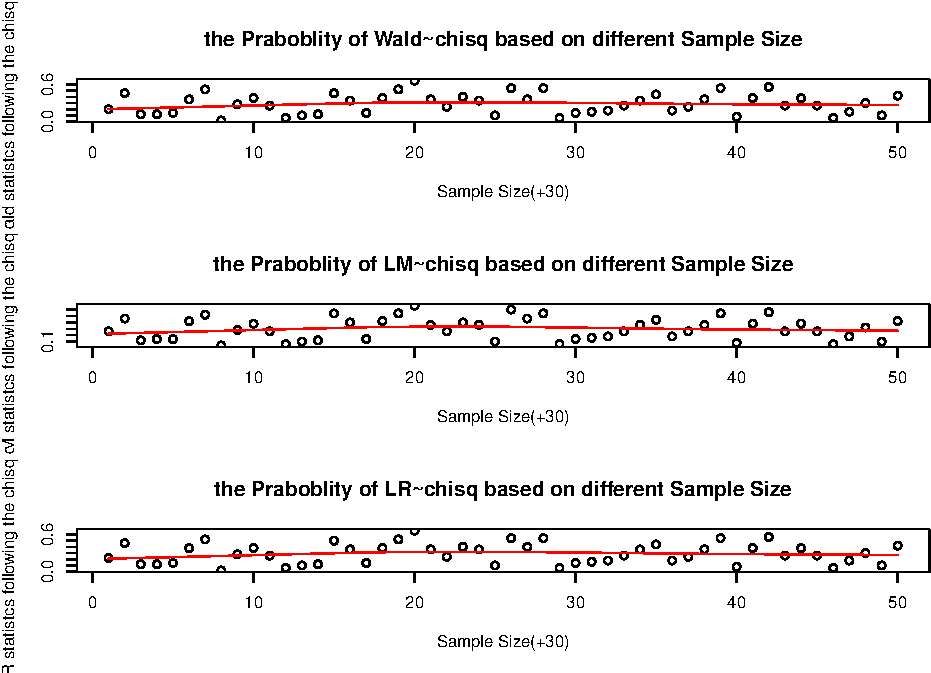
\includegraphics{BST169Coursework_project_answer_files/figure-latex/unnamed-chunk-1-1.pdf}

I use the WLS to estmate the model, which driectly avoid the potential
heteroscedacity. From the plots, I can find the each of these three test
statistics (in red line) show a convex function, which means when the
sample size increase the statistics will increase, which suggest me that
the statistics will follow chi-squred disrtribution. that is consistent
with the definition.


\end{document}
